

\input{settings_FM_template.tex}


\setbeamercovered{transparent=35}

\title[Editor konfiguračních souborů~Flow123d]{Editor konfiguračních souborů~Flow123d}
\subtitle{Diplomová práce}
\author[Bc. Tomáš Křížek]{Bc. Tomáš Křížek}
\institute[TUL]{Technická univerzita v Liberci}
\date{22.~března~2016}
\newcommand{\TextTitulniStranaPodLinkou}{\tiny
Studentská 2 {\color{FM_TUL} |} 461\,17 Liberec 2 {\color{FM_TUL} |} {tomas.krizek1@tul.cz} {\color{FM_TUL} |} 
\href{http://www.fm.tul.cz/}{www.fm.tul.cz}}

\begin{document}
%\setbeamertemplate{caption}{\insertcaption}


\begin{frame}
	\titlepage
\end{frame}

\begin{frame}
	\frametitle{Obsah}
	\begin{itemize}
		\item Zpracování konfiguračního souboru
		\item Specifikace formátu a validace
		\item Nápověda a automatické doplňování
		\item Uživatelské rozhraní
	\end{itemize}
\end{frame}

\begin{frame}[fragile]
	\frametitle{Zpracování konfiguračního souboru}
	\only<1>{
	\hspace*{-5pt}
\includegraphics[width=\textwidth]{../../img/data_structure_chain_1.pdf}\\
	}
	\only<2-6>{
	\hspace*{-5pt}
\includegraphics[width=\textwidth]{../../img/data_structure_chain_2.pdf}\\
	}
	\only<7-11>{
	\hspace*{-5pt}
\includegraphics[width=\textwidth]{../../img/data_structure_chain_3.pdf}\\
	}
	\only<12>{
	\hspace*{-5pt}
\includegraphics[width=\textwidth]{../../img/data_structure_chain_4.pdf}\\
	}
	\begin{minipage}[t]{0.45\textwidth}
	\begin{block}{Syntaxe a zpracování YAML}
	\begin{itemize}
		\item<3> primitivní datové typy, pole, záznamy
		\item<4> abstraktní záznamy
		\item<5> reference
		\item<6> pozice dat v původním souboru
	\end{itemize}
	\end{block}
	\end{minipage}
	\hspace{5pt}
	\begin{minipage}[t]{0.45\textwidth}
	\begin{block}{Autokonverze\vphantom{y}}
	\begin{itemize}
		\item<7> speciální zkrácený zápis polí či záznamů
		\item<8> autokonverze na pole
		\item<9> autokonverze na záznam
		\item<10> transpozice
		\item<11> libovolně vnořené
	\end{itemize}
	\end{block}
	\end{minipage}
\end{frame}

\begin{frame}[fragile]
	\frametitle{Specifikace formátu a validace}
	\vspace*{-10pt}
	\pause
	\begin{minipage}[t]{0.55\textwidth}
	\begin{block}{Specifikace formátu (IST)}
	\begin{itemize}[<+>]
		\item popis datové struktury
		\item informace pro validaci
		\item \textit{závislá na verzi Flow123d}
	\end{itemize}
	\end{block}
	\begin{block}{Validace\vphantom{y}}
	\begin{itemize}[<+>]
		\item syntaktické chyby
		\item sémantické chyby
		\item upozornění na možné překlepy
	\end{itemize}
	\end{block}
	\end{minipage}
	\hspace*{-10pt}
	\begin{minipage}[t]{0.35\textwidth}
	\vspace{55pt}
	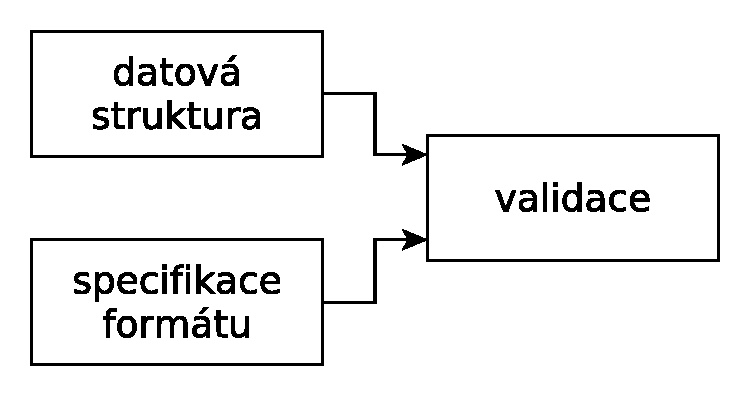
\includegraphics[width=1.4\textwidth]{../../img/validation_process.pdf}\\
	\end{minipage}
\end{frame}

\begin{frame}
	\frametitle{Validace}
	\vspace{15pt}
	\includegraphics[width=\textwidth]{img/validation.png}
\end{frame}

\begin{frame}[fragile]
	\frametitle{Nápověda a automatické doplňování}
	\vspace*{-20pt}
	\pause
	\begin{minipage}[t]{0.55\textwidth}
	\begin{block}{Nápověda}
	\begin{itemize}[<+>]
		\item kontextová dokumentace
		\item alternativa k~rozsáhlé referenční dokumentaci
	\end{itemize}
	\end{block}
	\begin{block}{Automatické doplňování}
	\begin{itemize}[<+>]
		\item doplňuje názvy klíčů, hodnoty výčtového typu, datové typy abstraktních záznamů
		\item citlivé na kontext
		\item filtrování v~průběhu psaní
	\end{itemize}
	\end{block}
	\end{minipage}
	\hspace*{-10pt}
	\begin{minipage}[t]{0.35\textwidth}
	\vspace{45pt}
	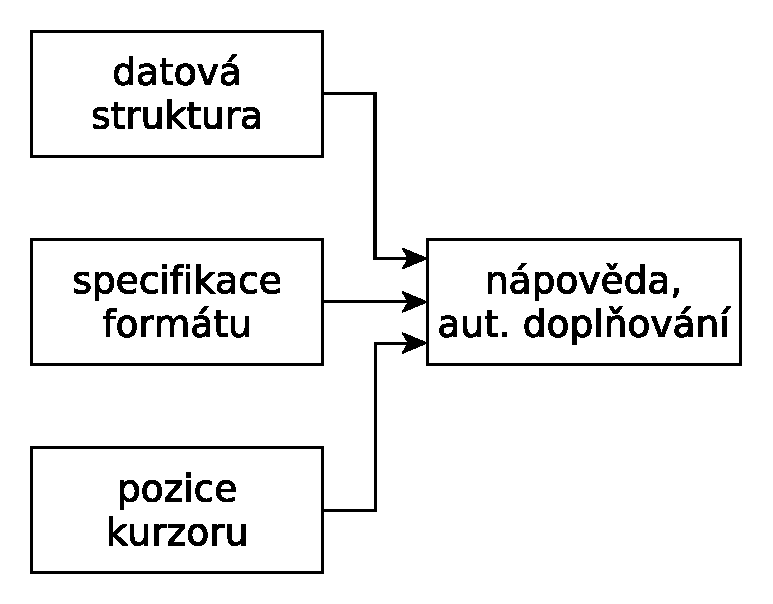
\includegraphics[width=1.4\textwidth]{../../img/documentation_autocompletion.pdf}\\
	\end{minipage}
\end{frame}
\begin{frame}
	\frametitle{Kontextová nápověda}
	\includegraphics[width=\textwidth]{img/doc_solver.png}
\end{frame}

\begin{frame}
	\frametitle{Kontextová nápověda}
	\vspace{10pt}
	\includegraphics[width=\textwidth]{img/doc_file.png}
\end{frame}

\begin{frame}
	\frametitle{Automatické doplňování}
	\hspace{65pt}
	\vspace{0pt}
	\includegraphics[width=0.45\textwidth]{img/autocompletion_all.png}\\
	\vspace*{15pt}
	\hspace{65pt}
	\includegraphics[width=0.45\textwidth]{img/autocompletion_filtered.png}\\
\end{frame}


\begin{frame}
	\frametitle{Shrnutí}
	\vspace{-5pt}
	\includegraphics[width=0.9\textwidth]{img/gui.png}\\
\end{frame}

\begin{frame}{}{}
\begin{center}
\huge Děkuji za pozornost.
\end{center}
\end{frame}


\end{document}
